
\begin{frame}
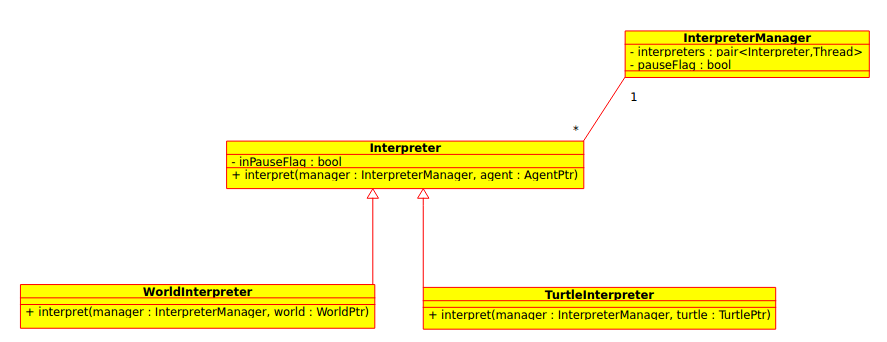
\includegraphics[scale=1]{doc/report/uml/interpreterUML.png}
\end{frame}

\begin{frame}
Rôle de l'interprète manager~:
\begin{itemize}
	\item Alerter des éventuelles pauses~;
	\item Création d'un monde avec les directives choisies~;
	\item Gérer les interpréteurs existants~;
	\item Stocker les couples threads-interprete créés.
\end{itemize}
C'est une sorte de gestionnaire d'interpréteurs.
\end{frame}

\begin{frame}
\note{L'interprete fonctionne de la manière suivante : lors de l'analyse d'un jeton, qui correspond à un nœud de l'arbre syntaxique, on analyse d'abord ses enfants (s'il y en a) puis ensuite le contenu du noeud courant.}
\end{frame}
